\section{Interaction-Preserving Motion Retargeting}
% \begin{table}[h!]
% \centering
% \small
% \renewcommand{\arraystretch}{1.3}
% \begin{tabularx}{\textwidth}{l *{4}{>{\centering\arraybackslash}X} l}
% \toprule
% Methods & Prevent Foot Skating & Non-penetration & Preserve Interaction w/ Object & Data Augmentation & Optimizer \\
% \midrule
% PHC & \no & \no & \no & \no & Gradient Descent \\
% GMR & \no & \no &\no & \no & Mink ~\cite{Zakka_Mink_Python_inverse_2025}\\
% VideoMimic & Soft penalty & Soft penalty & \no & \no & \makecell[t]{JAX Levenberg-\\Marquardt}\\
% IMMA & \yes & \yes & \no & \no & Lagrange Method\\
% \OmniRetarget (Ours) & \yes & \yes & \yes &\yes & SQP \\
% \bottomrule
% \end{tabularx}
% \caption{Comparison of retargeting methods across constraint enforcement, interaction preservation, data augmentation and optimization strategy.}
% \end{table}
\begin{table*}[t]
\centering
\footnotesize
\renewcommand{\arraystretch}{1.15}
\setlength{\tabcolsep}{4pt}
\begin{tabularx}{\textwidth}{l *{5}{>{\centering\arraybackslash}X} l}
\toprule
\textbf{Methods} & \textbf{Hard Kinematic Constraints} & \textbf{Interaction w/ Object} & \textbf{Interaction w/ Terrain} & \textbf{Data Augmentation} & \textbf{Optimization Method} \\
\midrule
IMMA~\cite{Nakaoka2012Interaction}  & \yes & \no & \no & \no & QP \\
PHC~\cite{Luo2023PerpetualHC} & \no & \no & \no & \no & Gradient Descent \\
GMR~\cite{ze2025twist}  & \no & \no & \no & \no & Mink~\cite{Zakka_Mink_Python_inverse_2025} \\
VideoMimic~\cite{videomimic}  & Soft Penalty & \no & \yes &\no & JAX L-M \\
\midrule
\textbf{\OmniRetarget (Ours)}  & \yes & \yes & \yes &\yes & Sequential SOCP \\
\bottomrule
\end{tabularx}
\caption{Comparison of prior retargeting methods across different aspects.}
\label{tab:retargeting_comparison}
% \vspace*{-0.4cm}
\end{table*}

%Levenberg-\\Marquardt

% IMMA relies on a complex, multi-stage pipeline: first, it optimizes keypoint positions to warp the interaction mesh from the human to the robot with minimal deformation; then, it solves an inverse kinematics problem to recover joint angles that best match the optimized keypoints. In later stages, additional hard constraints on the feet and waist are imposed to prevent foot slipping and ensure dynamic balancing. This sequential and fragmented approach produces dynamically consistent motions but 
 % \karen{This is what a reviewer might say: It sounds like the proposed method and IMMA can achieve the same thing and the only difference is that your method has a better implementation. I think we put too much effort in describing how IMMA works which dilutes the most important sentence: IMMA fails to enforce joint and velocity limits and does not support interactions with the environment and objects. We should say that right after "However". }.

\subsection{Interaction Mesh with Hard Constraints}
We leverage the interaction mesh \cite{Ho2010Spatial} to preserve spatial relationships between body parts, objects, and the environment. The interaction mesh is defined as a volumetric structure whose vertices consist of key robot or human joints together with points sampled from objects and the environment. By shrinking or stretching this mesh, we can warp human motion onto the robot while preserving relative spatial configurations and contact relationships.  

\textbf{Interaction Mesh Construction.}  
We construct the interaction mesh by applying Delaunay tetrahedralization \cite{si2005meshing} to user-defined key joint positions and randomly sampled object and environment points. To more accurately maintain contact relationships, we sample the object and environment surfaces more densely than the body joints. 
% \guanya{I think we need a humanoid example to illustrate it}
% \karen{Reviewer might wonder why we need to do Delaunay triangularization every frame. Even if we are solving frame by frame, the connectivity of the interactive mesh can remain across frames.}

\textbf{Optimization Objectives and Constraints.}
% To preserve the spatial relationships between the body parts, objects and terrains, our primary objective is to minimize the Laplacian deformation energy of the interaction meshes \cite{alexa2003differential, zhou2005large}. We define the set of all demonstration (retargeted) keypoints at frame $t$ as $\mathcal{P}_t^{\text{source}}$ ($\mathcal{P}_t$) \karen{I think there's a library that can make mathcal less curly}, which is the union of three distinct sets: points on the human (robot) $\mathcal{P}_t^{\text{human}} (\mathcal{P}_t^{\text{robot}}$), points on manipulated objects $\mathcal{P}_t^{\text{obj}}$, and points on the environment $\mathcal{P}_t^{\text{env}}$. The robot's keypoints are determined by its configuration $q_t$ via forward kinematics $f_i$ as $\mathcal{P}_t^{\text{robot}}(q_t) = \{f_i(q_t)\}$.
To preserve the spatial relationships between the body parts, objects and terrains, our primary objective is to minimize the Laplacian deformation energy of the interaction meshes \cite{alexa2003differential, zhou2005large} constructed from two corresponding sets of keypoints. The source set at frame $t$, $\mathcal{P}_t^{\text{source}}$, is composed of user-defined anatomical points on the human, and points randomly sampled on the manipulated object and the environment. The target set for the retargeted motion, $\mathcal{P}_t^{\text{target}}$, consists of corresponding anatomical points on the robot, the same manipulated object and environment points. Our method is relatively robust to the precise placement of these keypoints, requiring only a semantically consistent correspondence between the human and robot (e.g., hand to hand).
% \karen{I removed some unnecessary definitions of the obj and env sets because you only lightly use them in the later section and never define their members. You can introduce q later before equation 3.}

The Laplacian coordinate of the $i$-th keypoint $p_{t, i} \in \mathcal{P}_t$ is defined as the difference between the point and the weighted average of its neighbors $j \in \mathcal{N}(i)$:
\begin{equation}
    L(p_{t, i}) = p_{t, i} - \sum_{j \in \mathcal{N}(i)} w_{ij} \cdot p_{t, j},
\end{equation}
where $w_{ij}$ is the normalized weight and we omit $L$'s dependence on $\{p_{t, j}\}_{j\neq i}$ in the function definition for conciseness. For all our experiments, we use uniform weights, setting $w_{ij} = 1/|\mathcal{N}(i)|$. The deformation energy measures the change in these Laplacian coordinates between the source demonstration mesh $\mathcal{P}_t^{\text{source}}$ and the retargeted mesh $\mathcal{P}_t^{\text{target}}$: 
\begin{equation} \label{eq:deformation_energy}
    E_L = \sum_{p_{t,i} ^{\text{source}} \in \mathcal{P}_t^{\text{source}}, p_{t, i}^{\text{target}} \in \mathcal{P}_t^{\text{target}}} \|L(p_{t,i} ^{\text{source}}) - L(p_{t,i}^{\text{target}})\|^2.
\end{equation}

We seek the robot configuration $q_t$, consisting of the floating base pose (quaternion and translation) and all joint angles, that minimizes this deformation energy while satisfying a set of hard kinematic constraints. The robot's keypoints are determined by its configuration $q_t$ via forward kinematics $f_i$ as $p_{t, i}^{\text{robot}}(q_t) = f_i(q_t) \in \mathcal{P}_t^{\text{target}}$. At each time step, we solve the following constrained, nonconvex program:
 
\begin{subequations}
\vspace{-0.4cm}
\label{eq:interaction_mesh_opt}
    \begin{align}
    q_t^\star = \argmin_{q_t} \; & \sum_{i} \|L(p_{t,i} ^{\text{source}})-L(p_{t,i}^{\text{target}}(q_t))\|^2 + \|q_t - q_{t-1}\|_{Q}^2 \label{eq:interaction_mesh_cost}\\
    \text{s.t.} \quad & \phi_j(q_t) \geq 0, \forall j \label{eq:non-penetration_cstr}\\
    & q_{\min} \leq q_t \leq q_{\max} \label{eq:joint_lmt}\\
    & v_{\min} \cdot dt \leq q_t - q_{t-1} \leq v_{\max} \cdot dt \label{eq:vel_lmt} \\
    & p_t^{F} = p_{t-1}^{F}, \forall \text{stance foot}, \label{eq:foot_sticking_cstr} 
\end{align}
\end{subequations}
where $Q$ is a cost matrix that encourages temporal smoothness, $\phi_j$ denotes the signed distance function for the $j$-th collision pair, $q_{\text{min}} / q_{\text{max}}$ and $v_{\text{min}} / v_{\text{max}}$ are the configuration and velocity bounds, $p_t^{F}$ denotes the foot position. A foot is considered to be in the stance phase if its horizontal velocity in the source motion (in the xy-plane) falls below a threshold of 1 cm/s. This optimization program solves for a temporally consistent robot trajectory that minimizes interaction mesh deformation, subject to hard constraints for collision avoidance \eqref{eq:non-penetration_cstr}, joint and velocity limits \eqref{eq:joint_lmt}--\eqref{eq:vel_lmt}, and preventing foot skating \eqref{eq:foot_sticking_cstr}.

We solve \eqref{eq:interaction_mesh_opt} sequentially for each timestep using a customized Sequential Quadratic Programming (SQP)-style solver. Within each iteration, the objective \eqref{eq:interaction_mesh_cost} is quadratically approximated and the hard constraints \eqref{eq:non-penetration_cstr}--\eqref{eq:foot_sticking_cstr} are linearized around the solution from the previous iteration. To ensure temporal consistency and accelerate convergence, the optimization at frame $t$ is warm-started with the optimal solution from the previous frame ${q^\star_{t-1}}$. A key challenge in this formulation is computing derivatives involving the quaternion-based floating base orientation; our implementation leverages the automatic differentiation framework in Drake \cite{drake}, which correctly handles the differential geometry of rotations on the $\mathbb{S}^3$ manifold \cite{jackson2021planning}.
% , and will be open-sourced.

% Our interaction-mesh-based kinematic pipeline demonstrates significant generality. It is readily adaptable to various robot embodiments—including the Unitree G1, H1, and Booster T1 (Fig. \ref{fig:cross_embodiment}) —requiring only modifications to the keypoint correspondences in the interaction mesh and the robot's collision model. The framework is also versatile across diverse interaction types, including \textbf{robot-object} interactions using the OMOMO human-object interaction dataset \cite{li2023object}, \textbf{robot-terrain} interactions with our in-house captured MoCap data, and \textbf{robot-only} motion (flat terrain) from the LAFAN1 dataset \cite{harvey2020robust}.
Our interaction-mesh-based kinematic pipeline is highly general. It adapts to different robot embodiments, including the Unitree G1, H1, and Booster T1 (Fig.~\ref{fig:cross_embodiment}), by modifying only the keypoint correspondences in the interaction mesh and the robot’s collision model. It also supports diverse interaction types: \textbf{robot-object} interactions from the OMOMO \cite{li2023object}, \textbf{robot-terrain} interactions from in-house MoCap data, and \textbf{robot-only} motions on flat terrain from LAFAN1 \cite{harvey2020robust}.
\begin{figure}
\centering
\includegraphics[width=0.4\textwidth]{figures/robot-aug-crop.pdf}
	\caption{Cross-embodiment robot-object-terrain interaction. }
	\label{fig:cross_embodiment}
    % \vspace*{-0.6cm}
\end{figure}

% \begin{figure}
% \centering
% \includegraphics[width=0.48\textwidth]{figures/spatial_aug.png}
% 	\caption{Spatial augmentation. }
% 	\label{fig:spatial_aug}
%     \vspace*{-0.4cm}
% \end{figure}
% \begin{figure}
% \centering
% \includegraphics[width=0.48\textwidth]{figures/obj_shape_aug.png}
% 	\caption{Object shape augmentation. }
% 	\label{fig:obj_shape_aug}
%     \vspace*{-0.4cm}
% \end{figure}

\begin{figure*}
\centering
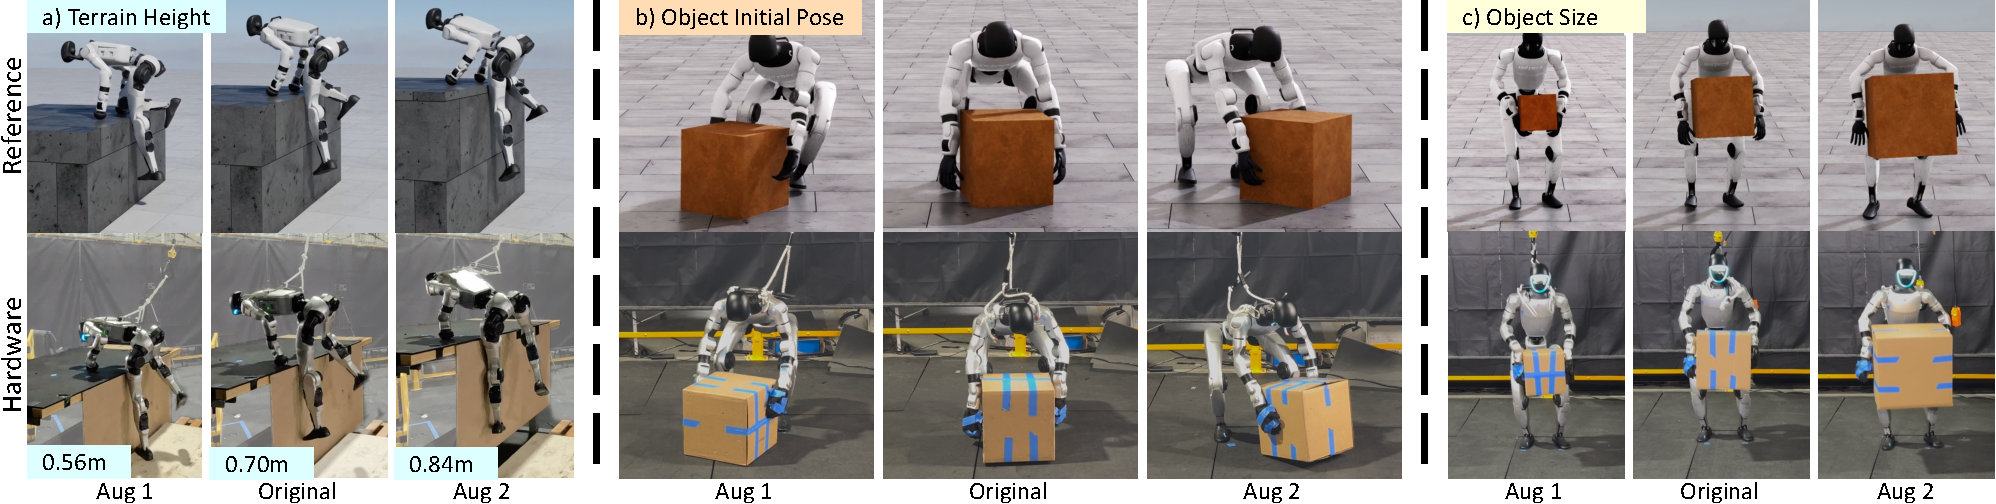
\includegraphics[width=\textwidth]{figures/aug-all-crop.pdf}
	\caption{\label{fig:aug} \OmniRetarget generates systematic variations of (a) terrain height, (b) object initial pose, and (c) object shape from a single human demonstration, with optimized motions in simulation (top) transferring consistently to hardware (bottom). }
	\label{fig:all_aug}
    % \vspace*{-0.4cm}
\end{figure*}

\subsection{Terrain, Object Shape and Spatial Augmentation}
\label{sec:aug}
A key advantage of our framework is its capability for systematic data augmentation, which eliminates the need for collecting numerous, repetitive demonstrations with minor spatial variations. Our method can transform a single human demonstration into a rich and diverse dataset by parametrically altering object configurations, shapes, or terrain features. For each new scenario, we re-solve the optimization problem with fixed $\mathcal{P}_t^{\text{source}}$ and augmented $\mathcal{P}_t$: minimizing the interaction mesh deformation finds a new, kinematically valid robot motion $\{q_t\}$ that preserves the essential spatial and contact relationships of the original interaction.

\textbf{Robot-Object.}
We generate diverse interactions by augmenting both the object's spatial configuration and its shape. 
% We apply rotations and translations to the object's initial pose (Fig. \ref{fig:spatial_aug}), which is then smoothly annealed into the nominal trajectory via an exponential schedule detailed in \eqref{eq:aug_obj_traj}, and scale its dimensions (Fig. \ref{fig:obj_shape_aug}) 
We apply translations and rotations to modify the object's initial pose (Fig. \ref{fig:all_aug}b) and blend the new initial pose with the original object motion via interpolation with an exponential schedule detailed in \eqref{eq:aug_obj_traj}. 
In addition, we scale the three dimensions of the object (Fig. \ref{fig:all_aug}c). A critical component of this process is constructing the interaction mesh in the object's local frame, which ensures that the robot's interacting body parts naturally follow the object's transformation (Sec. \ref{sec:im_in_obj_frame}). 

However, this alone can lead to trivial augmentations where the entire robot undergoes a rigid transformation along with the object. To generate more meaningful data diversity, we introduce cost terms and constraints that anchor parts of the robot's body to the nominal trajectory $\{\bar q_t^\star\}$. For instance, in a pick-up task, we encourage the robot to discover new upper-body coordination by penalizing lower-body deviations from the original motion:
\begin{equation}
    \|q_t - \bar q_{t}^\star\|_W,
\end{equation}
where $W$ heavily penalizes the lower-body entries, constraining the initial foot poses to match the nominal trajectory
\begin{equation}
    p_0^{F} = \bar p_{0}^{F \star} \quad \text{ for left and right feet}.
\end{equation}
These added objectives prevent the optimization from collapsing to a simple rigid transform of the nominal trajectory and instead produce genuinely new and diverse interactions.

\textbf{Robot-Terrain.}
We generate diverse terrain scenarios by scaling environmental features, such as varying the platform height and depth (Fig. \ref{fig:all_aug}a), and introducing additional constraints. For instance, to encourage stable ground contact when the terrain is elevated, we uniformly sample a grid of points on the ground surface into the interaction mesh.

